In this section, data modelling of the system including definitions of data domain, data fields for each domain, and relation between domains will be performed in the first place. In the following subsection, APIs corresponding to related operations on data models will be assigned.

\subsection{General Data Model}


\subsubsection{ Data Domain }
In general, data in the system could be divided into 4 primary domains:

\begin{enumerate}
\item
\textbf{User}: personal information as well as user identifier for accessing the system.
\item
\textbf{Course}: a container with own course information as well as collection of questions classified to this context.
\item
\textbf{Question}:  data with information of questions submitted by users.
\item
\textbf{Answer}: data with information of answers, also has graphical data within the data model.

\end{enumerate}

Users are able to assess the contributions made by other users and mark it as useful or useless, which will affect the contributions' oder priority while rendering the views. Voters should also be aware of what kind of vote he has marked to the contribution. Therefore, additional 2 data models \textbf{VoteAnswer} and \textbf{VoteQuestion} should also be considered. 

The relation between domains is illustrated in the following figure \ref{ata-domain-relation}. Each data modal has an unique identifier, which is referenced in another data model when they have a connection. 

\begin{figure}[!htbp]
  \centering
    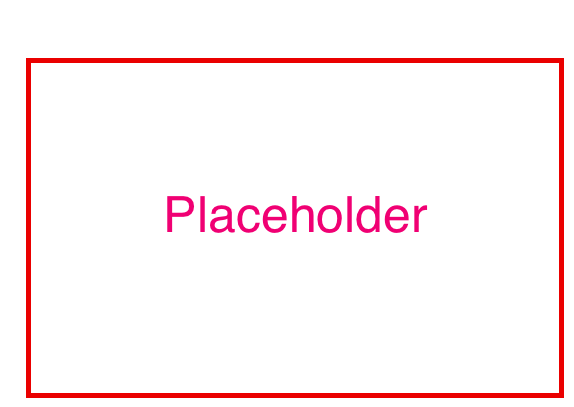
\includegraphics[width=0.6\textwidth]{Figures/placeholder.png}
  \caption{placeholder}
  \label{fig:data-domain-relation}
\end{figure}
% relation pic
% Belonging!!! User->Course->Question->Answers!
% PowerDesigner - Tool!


\subsubsection{ Data Fields }

More detailed definition and description of fields in each data model should be made for a better understanding of the structure as well as behaviour of a data model. Tabel \ref{data-field-table} describes key fields of general domains.


\begin{table}[]
\centering
\begin{tabularx}{\textwidth}{@{}llX@{}}
\toprule
Domain                    & Field           & Description                                                                                    \\ \midrule
\multirow{4}{*}{User}     & email           & unique identifier of an user for authentification, also as contact way to user.                \\
                          & password        & string for user authentication to prove identity or access approval                            \\
                          & username        & user identifier shown to other users                                                           \\
                          & isTutor         & flag which determines if the user is a student or tutor                                        \\ \midrule
\multirow{4}{*}{Course}   & name            & name of the course                                                                             \\
                          & desc            & description of the course                                                                      \\
                          & creator         & id of the user(tutor) who created this course                                                  \\
                          & code            & unique code for quick search purpose which is generated automatically as the course is created \\ \midrule
\multirow{5}{*}{Question} & title           & title of the question                                                                          \\
                          & content         & content of the question                                                                        \\
                          & course          & id of the the course to which the question belongs                                             \\
                          & vote            & vote count of the question                                                                     \\
                          & creator         & id of the user who submitted this question                                                     \\ \midrule
\multirow{5}{*}{Answer}   & content         & content of the answer                                                                          \\
                          & question        & id of the question for which the answer is made                                                \\
                          & quoted          & id of the original question which is quoted                                                    \\
                          & vote            & vote count of the answer                                                                       \\
                          & creator         & id of the submitter                                                                            \\ \midrule
\multirow{3}{*}{Vote}     & type            & enum values of up-voting or down-voting actions                                                \\
                          & handler         & id of the hander                                                                               \\
                          & question/answer & id of the question/answer to which the vote action is applied                                  \\ \midrule
\end{tabularx}
\caption{Fields for Each Data Domain}
\label{table:data-field-table}
\end{table}


\subsection{RESTful API Definitions}

As mentioned in section xxx, RESTful architecture is a an excellent technical choice for data transferring. Because of its simplicity and clear semantic description of HTTP methods comparing to other protocols such like SOAP, it will dramatically simplify and clarify our data transmission services. 

\subsubsection{ Mapping of HTTP methods to data model behaviour }
The data model defined above can directly map to the definition of resources in RESTful. The HTTP methods on each resource domain can also represent the data model behaviours, \textbf{\textit{User Model}} is taken as an example: 
\begin{table}[!htbp]
\centering
\begin{tabularx}{\textwidth}{@{}lX@{}}
\toprule
Method        & {Operation of data model collection }                            \\ \midrule
GET           & {Query and return a specific user from user model collection.}   \\
POST          & {Create a new user entry and insert into user model collection.} \\
PUT           & {Update a specific user in user model collection.}               \\
DELETE        & {Delete a specific user in user model collection.}               \\ \bottomrule
\end{tabularx}
\caption{HTTP methods on User resource}
\label{table:http-method-on-user-resource}
\end{table}

In table \ref{http-method-on-user-resource}, resource entry in persistent storage can be executed with specific action while requesting resource URI through different HTTP methods. A semantic description of connection between \gls{CRUD} and HTTP methods on RESTful will make the data transmission services more understandable and unified.

\subsubsection{ General RESTful API Definitions }

Requesting a specific resource can only succeed through its \gls{URI}, through which the client and server-side could connect to each other actually. Therefore, a definition of APIs which describes \gls{URI} of the resources and its functional responsibility should be proposed in the first place.


\begin{enumerate}
\item
\textbf{User Authentication}: the major actions of user authentication include signup, login, logout. To protect the user information, POST method which doesn't expose information via the URL, is highly recommended.

\begin{table}[!htbp]
\centering
\begin{tabularx}{\textwidth}{@{}llX@{}}
\toprule
URI          & Method & Description                                                  \\ \midrule
/auth/login  & POST   & User login action, request with login information.           \\
/auth/signup & POST   & User signup action, request with registration information.   \\
/auth/logout & GET    & User logout action, no data submission is needed.            \\ \bottomrule
\end{tabularx}
\caption{User Auth APIs}
\label{table:user-auth-apis}
\end{table}

\item
\textbf{Courses}: acquisition of courses and new submission of a course is possible. In addition, \gls{CRUD} operations on a specific course should also be achieved through a single URI with various HTTP methods.

\begin{table}[!htbp]
\centering

\begin{tabularx}{\textwidth}{@{}llX@{}}
\toprule
URI                 & Method         & Description                                                                                                          \\ \midrule
/courses            & GET/POST       & request the whole collection of courses; create course with data submitted \\
/courses/:courseId & GET/PUT/DELETE & request, modify, remove specific entry of course                                                                     \\ \bottomrule
\end{tabularx}
\caption{Course Resource APIs}
\label{table:course-resource-apis}
\end{table}

\item
\textbf{Questions}: in a real sense question resource is attached to course resource. According to the best practise of RESTful API design [reference xxx], question resource could be touched under course URI, \textit{/courses/:courseId/questions/:questionId}. But in the real world, question resource has its own collection, and \textit{questionId} is the unique identifier, through which a specific question entry could be selected without using  
\textit{courseId}. So an optimized conception is simply using \textit{/questions} as URI instead. And pass \textit{courseId} as a query parameter while requesting collection of question entries under a specific course. 
\begin{table}[!htbp]
\centering

\begin{tabularx}{\textwidth}{@{}llX@{}}
\toprule
URI                                   & Method         & Description                                                                                                                                                 \\ \midrule
/questions?courseId=:id               & GET/POST       & request the whole collection of questions belonging to a specific course; create question under a specific course \\
/questions/:id                & GET/PUT/DELETE & request, modify, remove specific entry of question                                                                                                          \\
/questions/:id/vote/:type      & POST          & vote actions with different vote types applied to specific question  \\ \bottomrule
\end{tabularx}
\caption{Question Resource APIs}
\label{table:question-resource-apis}
\end{table}


\item
\textbf{Answers}: the general API design of answer is totally same as the approach applied in question resource. A independent API for voting functionality should also be designed. And multiple possibilities of vote types could also be passed through the API.

\begin{table}[!htbp]
\centering

\begin{tabularx}{\textwidth}{@{}llX@{}}
\toprule
URI                                 & Method         & Description                                                                                                                                                 \\ \midrule
/answers?questionId=:id             & GET/POST       & request the whole collection of answers belonging to a specific question; create answer under a specific question\\
/answers/:id                        & GET/PUT/DELETE & request, modify, remove specific entry of answer                                                                                                            \\
/answers/:id/vote/:type             & POST           & vote actions with different vote types applied to specific answer                                                                                           \\ \bottomrule
\end{tabularx}
\caption{Answer Resource APIs}
\label{table:answer-resources-apis}
\end{table}

\end{enumerate}

Once all APIs with different HTTP methods are defined, a more concrete data structure over the APIs between two sides should be promised and confirmed. By following defined APIs and promised data structure, developments on both client and server-side could be executed parallelly.

\subsection{WebSocket Definitions} \label{subsection:websocket-definition-data-concept}

As the requirements defined in section \ref{sec:aims}, users could be informed as new question is posted or the order of answers with rating priority changes. Basically, only two different types of listeners are needed in this case: one for listening to the new questions under a specific class and one for responsive order of answers under a specific question. With WebSocket, URI should also be defined as an identifier for the persistent connection between client and server. And different events within a connection of one URI should also be designed. Table \ref{table:websocket-def} defines these two WebSocket specifications.

\begin{table}[!htbp]
\centering
\begin{tabularx}{\textwidth}{@{}llX@{}}
\toprule
URI                       & Event           & Response                           \\ \midrule
/ws/courses/            & questions-changed       &  data of new question posted by others \\
/ws/questions/          & answers-changed      &  data of answers in new order          \\ \bottomrule
\end{tabularx}
\caption{Answer Resource APIs}
\label{table:websocket-def}
\end{table}

